%!TEX root = parita-msc.tex

\chapter{Related Work}
\label{chap:relwork}
\begin{doublespace}

This chapter includes the theoretical and conceptual information that builds the foundation for this thesis.
Broadly, this chapter covers the semantic web and linked open data from the two perspectives of technology and usability. 

%The study of semantic web and related concepts has been successful in drawing the interest of many researchers, data scientists, and web designers. But, topics like semantic web and linked data are still too wide to be discovered and explored. There are still some related areas that have not been explored yet. The topic of research here is a small attempt at one of those unexplored topics. 


\section{The Web}

The idea of the Web, as per Berners-Lee~\cite{bernersreadings}, was derived from a positive experience of a small \say{home-brew}, a personal hypertext system. This \say{home-brew} system was used to keep track of personal information on a distributed project. The Web can be used independently for multiple projects that can be later integrated with unique relationships among them using the newly shaped information to represent the new state of linked knowledge.
The web was first designed by Berners-Lee in 1989\footnote{https://www.w3.org/History/1989/proposal.html} while working at the \ac{cern}. The web, today, has advanced more, evolved, and progressed to develop multiple versions. Different versions of the Web were designed and declared as generations like Web 2.0, Web 3.0, and Web 4.0. Web 2.0 has been accepted and included for a long time now, Web 3.0 is comparatively new, whereas Web 4.0 is at the initial stage of research and application. An idea of different versions of the web can be derived from Figure~\ref{fig:2.1}.
\begin{figure}[htp]
    \centering
    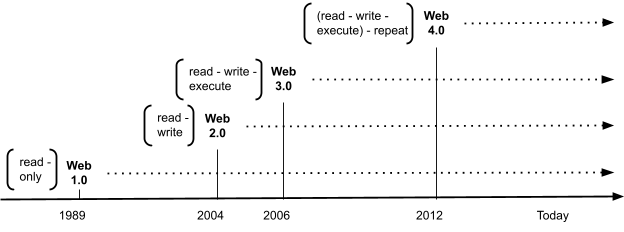
\includegraphics[width=15cm]{images/ch2/Figure1.png}
    \caption{Different Versions of the Web, according to Aghaei et al.~\cite{aghaei2012evolution}}
    \label{fig:2.1}
\end{figure}

The first version of the Web designed in 1989, as per Aghaei et al.~\cite{aghaei2012evolution}, was read-only. 
The users of the web browsers for Web 1.0 could only read the information present on the web pages. The right to modify the contents of the web page was only with the website owners. 
In 2004, Dale Dougherty at O'Reilly Media~\cite{aghaei2012evolution} formally designed an improved version of Web 1.0 and called it Web 2.0 where the users had the liberty to read as well as modify the data on the web. The web browsers for this generation of the web offered comparatively more features than Web 1.0, making the websites more efficient and engaging. Features like web designing, creation, and modification also helped Web 2.0 in the introduction of blogs, vlogs, wikis\footnote{www.wiki.org/wiki.cgi?WhatIsWiki} and social networking technologies~\cite{harris2009web}.

\section{Semantic Web}

In 2006, John Markoff~\cite{aghaei2012evolution} introduced the new read-write-execute web as Web 3.0 in New York Times. Structured datasets and the links between them are used for the successful working of Web 3.0, also known as the Semantic Web. The web pages for the semantic web can be written using \ac{html} and \ac{rdf} as it is the web of data, contrary to the web of documents, where the web pages were written using \ac{html} and the links were described using hyperlinks. In the web of data, arbitrary things can be expressed using links to represent the relationship between two entities, as shown in Figure~\ref{fig:2.2}.

\begin{figure}[htp]
    \centering
    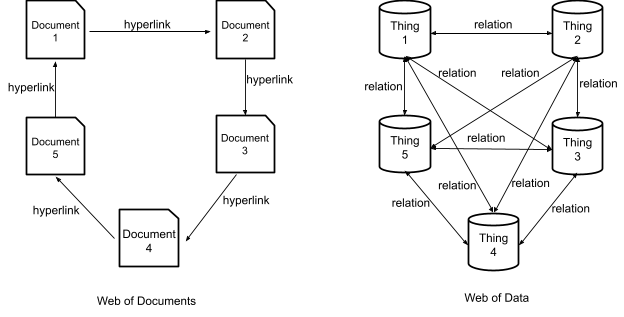
\includegraphics[width=15cm]{images/ch2/Figure2.png}
    \caption{The Web to Semantic Web, according to Aghaei et al.~\cite{aghaei2012evolution}}
    \label{fig:2.2}
\end{figure}

The latest generation of web that is still at its research and development stage is Web 4.0 which is supposed to be read-write-execute with the property of concurrency~\cite{choudhury2014}. This version of the web is intended to work with artificial intelligence to give users an exceptional quality of experience. While describing how Web 4.0 would be, Berners-Lee~\cite{bernerslee1999weaving}
stated \say{if \ac{html} and the Web made all the online documents look like one huge book, \ac{rdf}, schema, and inference languages will make all the data in the world look like one huge database}.
\subsection{The Semantic Web Stack}
\par The Semantic Web Stack
\footnote{https://en.wikipedia.org/wiki/Semantic\_Web\_Stack} is also known as Semantic Web Cake or Semantic Web Layer Cake. The stack represents the architecture of semantic web. Figure~\ref{fig:2.3}\footnote{https://www.w3.org/2001/12/semweb-fin/w3csw} shows how semantic web principles are implemented in the layers of technologies.
\begin{figure}[htp]
    \centering
    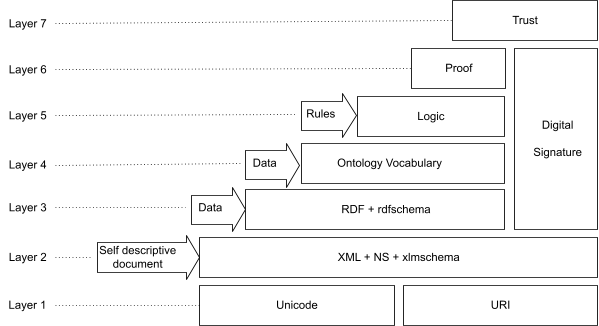
\includegraphics[width=15cm]{images/ch2/Figure3.png}
    \caption{Semantic Web Stack}
    \label{fig:2.3}
\end{figure}
\par The layers in the stack consist of different technologies. Going from the lowest level to the top level, the technologies are Unicode and \ac{uri}; \ac{xml}, NS and xmlschema; \ac{rdf} and rdfschema; Ontology vocabulary; Logic; Proof; and Trust. Digital signatures are used as security at different levels. The layers belong to three different groups, namely, self-descriptive document, data and rules.
\section{Linked Open Data}
\par According to Berners-Lee et al.~\cite{aghaei2012evolution}, \say{Semantic web is not limited to publication of data on the web; it is about making links to connect related data.} The concept of Linked Open Data\footnote{https://www.ontotext.com/knowledgehub/fundamentals/linked-data-linked-open-data/} is an amalgamation of two technologies, Linked Data and Open Data. GraphDB\footnote{https://www.ontotext.com/knowledgehub/fundamentals/linked-data-linked-open-data/} by Ontotext, an \ac{rdf} database, is an example of \ac{lod}. GraphDB promotes knowledge-discovery and efficient data-driven analytics by linking large datasets from distinct sources to Open Data.
\subsection{Linked Data}
\par The relationships shared among the data from different sources on the web are equally important as the access to the data for efficient working of the semantic web. The technique used to manage these datasets and their relationships is referred to as Linked Data. In other words, Linked Data\footnote{https://www.w3.org/wiki/LinkedData} can be termed as a set of various techniques of publishing structured data on the web. The \ac{w3c} standards and various semantic web technologies handle the distribution and engagement of the structured data across the web to aggregate the data available on the web into one huge database~\cite{bernerslee1999weaving}.
\par In 2006, Berners-Lee~\cite{bizer2009linked} framed four basic rules (mentioned in section \ref{principles}) to publish and connect the structured datasets across the web. This set of rules was termed as Linked Data principles. A brief description of these principles is as follows:
\begin{enumerate}
  \item Use \ac{uri}s as names for things:
  \par The web identifiers, the (\ac{uri}s) should be used to give unique names to all the entities (or things) on the web. \ac{uri} of an entity can be used to understand that the entity in this dataset is the same as the other entity in a disparate dataset. 
  \item Use \ac{http}\footnote{Both \ac{http} and \ac{https}} \ac{uri}s to look up for those names:
  \par The \ac{http}/\ac{https} protocols allow easy retrieval of resources. Hence, along with \ac{uri}s, either of the protocols can be used to search things (entities) easily. This promotes the publication of data on the web and its addition to the global data space.
  \item Provide useful information, using the standards (\ac{rdf}\footnote{includes all the standards belonging to \ac{rdf} family}, \ac{sparql}) to look up for a \ac{uri}:
  \par When an entity is searched using the \ac{uri} associated with it, it is beneficial to use standards like \ac{rdf} and \ac{sparql} to query the datasets. \ac{rdf} is a framework used for graphical representation of publication and distribution of data on the web, as described in detail in section~\ref{section:rdf}. On the contrary, \ac{sparql} is a query language used for retrieval and manipulation of data (in \ac{rdf} format) on the web. It also helps with the information on relationships related to the data being searched.
  \item Include links to other \ac{uri}s to discover more thing:
  \par In the semantic web, links between two entity defines the relationship using the basic entity-relationship model. Using links for \ac{uri}s of the entities promotes interconnection of the data and search of things on the web. Connecting new data to already existing entities increases the reuse and interlinking within the domain and creates a computer-understandable network.
\end{enumerate}
\par Publishing data on the web as per linked data principles can benefit the data providers by allowing them to use one global space to add all their data. An \ac{rdf} data model and \ac{uri}s are used by the linked data to name the things (entities). The linked datasets publish and locate the class-object data which in turn is accessed using the \ac{http}/\ac{https} and maintains the connection among them~\cite{bauer2011linked}. 
\par A wide network of structured data, from a variety of domains, on the web has been formed obeying the principles of linked data by Berners-Lee. This has resulted in the formation of a huge database of structured linked data on the web which has further led to the concept of the \ac{lod} Cloud. The \ac{lod} cloud is a set of publicly~\cite{berners1998universal} accessible/available linked datasets.
\subsection{Linked (Open) Data}
\par According to a handbook\footnote{https://opendatahandbook.org/guide/en/what-is-open-data/} by the Open Knowledge Foundation, \say{Open Data is data that can be freely used, re-used and redistributed by anyone - subject only, at most, to the requirement to attribute and share-alike}. To make open data available to everyone on the web, the data don't need to be interlinked. Important features of open data are:
\begin{itemize}
  \item Availability and access: the data should be available on the web. The users should be able to access the data easily by downloading them over the internet. It should be easy to access and modify the data.
  \item Re-use and redistribution: the data on the web must have permissions to re-use and redistribute in combination to other datasets.
  \item Universal participation: the data should be available to use, re-use, and redistribute for all the users without any discrimination to an individual or a group.
\end{itemize}
\section{Resource Description Framework} \label{section:rdf}
\par The \ac{rdf}, initially designed as a metadata data model, is a computer-understandable specification written in a particular format. According to a proposal by \ac{w3c}\footnote{https://www.w3.org/TR/PR-rdf-syntax/Overview.html}, \ac{rdf} plays an important role in their \say{Semantic Web Vision}. \ac{rdf} describes an entity (or resources) and the relationships among them on the web using basic data models like the \ac{er} model.
\par \ac{rdf} is a \ac{w3c}\footnote{https://www.w3schools.com/xml/xml\_rdf.asp} specification for describing resources on the web. \ac{rdf} uses \say{properties} and \say{property values} to describe the resource which is identified by web identifiers called \ac{uri} (section~\ref{subsection:uri}). There are three types of objects in \ac{rdf}, namely, resources, properties, and statements. Each data object in a dataset on the web is considered a resource and is named using a \ac{uri} with an optional ID. To search for the resources on the web, the resources must be named using the \ac{http}/\ac{https} \ac{uri}s. The \ac{w3c} has defined the \say{rdf:type} property to represent the \say{object of one or more classes}~\cite{cyganiak2014rdf}. Resources are described by their characteristics, called \say{property}. The object of \ac{rdf} that is used to combine a resource with a property of its value is a \say{statement}. A statement, in general terms, can be seen as building blocks of a statement in English, which are a subject, an object, and a predicate. An object in a statement can be either a property value, a resource, or a literal. \ac{rdf}, according to Swick and Lassila~\cite{beckett2004rdf}, can be represented in three ways:
\begin{enumerate}
  \item Using \ac{xml}: an \ac{rdf}/\ac{xml} document
  \item As triples: subject-predicate-object form
  \item In graphical form
\end{enumerate}
\par Figure~\ref{fig:2.4} shows an example of an \ac{rdf}/\ac{xml}\footnote{\ac{rdf} written using \ac{xml}} document. The resource being described is \say{https://www.semanticweb.org/pda324/ontologies/survey} and \say{Survey Details} is the property value. The document consists of various \ac{xml} tags enclosed between the angular brackets (\say{<} and \say{>}). An \ac{rdf}/\ac{xml} document starts and ends with <rdf : \ac{rdf}> and </rdf : \ac{rdf}> respectively. <rdf : Description> consists of the elements that are responsible for the creation of the statement. Description tag holds an identification for the resource.
\begin{figure}[htp]
    \centering
    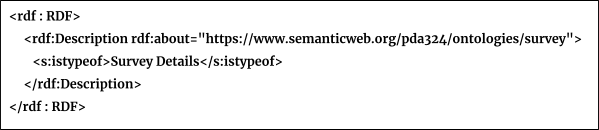
\includegraphics[width=15cm]{images/ch2/Figure4.png}
    \caption{An Illustration of Code in an RDF/XML Document}
    \label{fig:2.4}
\end{figure}
\par Figure~\ref{fig:2.5} shows an example of an \ac{rdf} as a triple. An \ac{rdf} triple, generally, follows subject-predicate-object format. For the illustration in the figure, the subject is \say{https://www.semanticweb.org/pda324/ontologies/survey}, predicate is \say{includes} and the object is \say{Survey Details}.
\begin{figure}[htp]
    \centering
    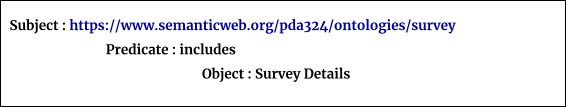
\includegraphics[width=15cm]{images/ch2/Figure5.png}
    \caption{An Example of an \ac{rdf} Triple}
    \label{fig:2.5}
\end{figure}
\par Figure~\ref{fig:2.6} show an \ac{rdf} in graphical format. Resource is indicated using an oval shape and a rectangle is used to represent a property value. A connector (an arrow) is used to represent a property to show that property (predicate) connects the resource (subject) with the value (object).
\begin{figure}[htp]
    \centering
    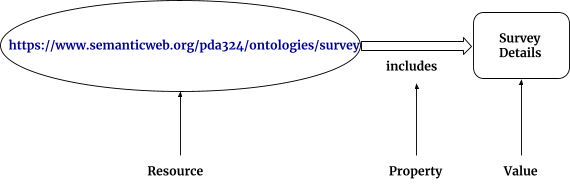
\includegraphics[width=15cm]{images/ch2/Figure6.png}
    \caption{Graphical Representation of an \ac{rdf}}
    \label{fig:2.6}
\end{figure}
\par The subject and object of the triples of \ac{rdf} act as nodes in the graph. In addition to \ac{rdf}/\ac{xml} documentation, the \ac{rdf} data model has a variety of serialization formats such as N-triples, which is a line base format where an \ac{rdf} triple is used to represent each line~\cite{beckett2014rdf}; \ac{turtle}; \ac{n3}, which is a subset of Turtle and N-Quads, which is an extension of N-Triples (line based) and adds a graph label to each line that allows multiple graph encoding~\cite{cyganiak2008n}.
\begin{table}[h!]
\centering
\begin{tabular}{| l | l |} 
 \hline
 Class/Property & Description  \\ 
 \hline
 rdfs:Resource & All things described by \ac{rdf} are called resources  \\ \hline
 rdfs:Class & The class of resources that are \ac{rdf} classes \\ \hline
 rdf:Property & The class of \ac{rdf} properties. It is an instance of rdfs:Class  \\ \hline
 rdfs:Literal & The class of literal values like integers and strings  \\ \hline
 rdfs:Datatype & The class of datatypes. All the objects of this class \\ & correspond to the \ac{rdf} model of datatype  \\ \hline
 rdf:HTML & The class of \ac{html} literal values and subclass of rdfs:Literal  \\ \hline
 rdfs:range & An instance of rdf:Property that is used to state that the \\ & values of a property are instances of one or more classes   \\ \hline
 rdfs:domain & An instance of rdf:Property that is used to state that any \\ & resource that has a given property is an instance of one or \\ & more classes. \\ \hline
 rdf:type & An instance of rdf:Property that is used to state that a \\ & resource is an instance of a class  \\ \hline
 rdfs:subClassOf & An instance of rdf:Property that is used to state that all the \\ & instances of one class are instances of another  \\ \hline
 rdfs:label & an instance of rdf:Property that may be used to provide a \\ &  human-readable version of a resource's name  \\ \hline
 rdfs:subPropertyOf \ \ & An instance of rdf:Property that is used to state that all \\ & resources related by one property are also related by another  \\ 
 \hline
\end{tabular}
\caption{Commonly used Classes and Properties of RDFS}
\label{table:2.1}
\end{table}
\par \ac{rdfs}, according to McBride~\cite{mcbride2004resource}, was introduced by the \ac{w3c} as a technique to define resource types and property names. The data publishers can use \ac{rdfs} to define various vocabularies in an \ac{rdf} model. Some of the commonly used \ac{rdfs} classes and properties\footnote{https://www.w3.org/TR/rdf-schema/} along with their description are listed in Table~\ref{table:2.1}~\cite{mcbride2004resource}.
\par Figure~\ref{fig:2.7} shows a graph for the representation of \ac{rdfs} for a comparatively complex and abstract example based on \ac{rdf} Primer~\cite{manola2004rdf}. The graph has been drawn for the following statement:
\emph{\begin{center}
    Romeo and Juliet is written by William Shakespeare.
\end{center} }
\par Figure~\ref{fig:2.7} is the graphical representation of an \ac{rdf} with schema as well as data. In the graph, the rdf:type of \say{Romeo and Juliet} is \say{Play} which in turn is an rdf:subClassOf \say{Literature}. Also, the rdf:type of \say{William Shakespeare} is \say{Person} which, further, is an rdfs:range of \say{is written by} of rdfs:domain \say{Literature}.
\begin{figure}[htp]
    \centering
    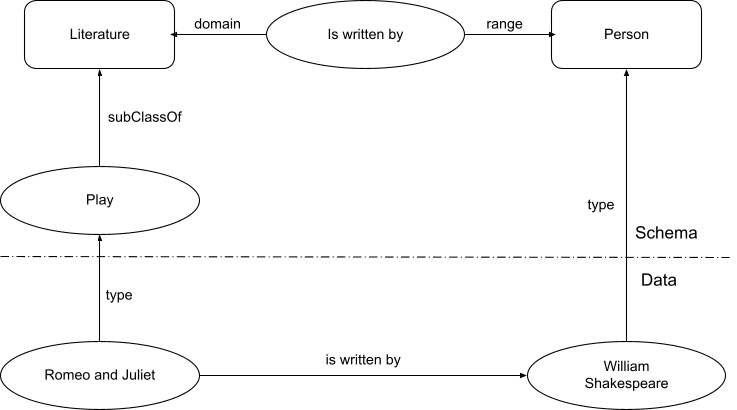
\includegraphics[width=15cm]{images/ch2/Figure7.png}
    \caption{Graphical Representation of an RDFS for a Comparatively Complex Illustration, after McBride~\cite{mcbride2004resource}}
    \label{fig:2.7}
\end{figure} 
\par The actual \ac{rdf} looks quite different from the previous example (Figures~\ref{fig:2.4}, ~\ref{fig:2.5}, ~\ref{fig:2.6} and ~\ref{fig:2.7}). For the representation of an actual \ac{rdf}, consider Figure~\ref{fig:2.8} for the corresponding English statement. \say{http://www.semanticweb.org/survey.html} is a subject \ac{uri} with respondent and Robert James having \ac{uri}s as \say{http://xyz.org/1/respondent} and \say{http://www.semanticweb.org/responseID/1234} respectively. The example represents a survey system which has responses as well as respondents and related details as a part of the environment.
\begin{figure}[htp]
    \centering
    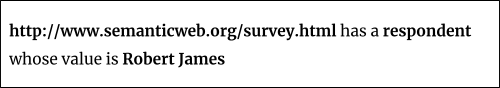
\includegraphics[width=15cm]{images/ch2/Figure8.png}
    \caption{English Statement for an Example of Actual \ac{rdf}}
    \label{fig:2.8}
\end{figure}
\par In the form of \ac{rdf} triple, the statement in Figure~\ref{fig:2.8} can be represented as shown in Figure~\ref{fig:2.9}. \ac{uri} is assigned to the subject survey.html and to the object which is the response with responseID 1234 which corresponds to the property value Robert James. A \ac{uri} is also assigned to the predicate (respondent).
\begin{figure}[htp]
    \centering
    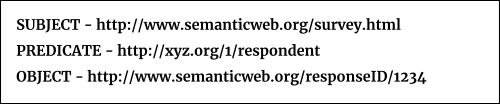
\includegraphics[width=15cm]{images/ch2/Figure9.png}
    \caption{\ac{rdf} Triple for English Statement in Figure~\ref{fig:2.8}, after \ac{rdf} Primer~\cite{manola2004rdf}}
    \label{fig:2.9}
\end{figure}
\par Figure~\ref{fig:2.10} shows a graphical representation of the \ac{rdf} triple in Figure~\ref{fig:2.9}. The subject and the object are two entities and the predicate being the third entity acts as a connector between them. Considering an entity-relationship data model, the predicate can be treated as a relationship shared by the subject and the object. There can be more details added to the system, that is, more statements can be added which are in relation to the one in Figure~\ref{fig:2.8}. Suppose the new statement added is:
\begin{center}
\par \emph{http://www.semanticweb.org/survey.html} has a \emph{date} with value \emph{Sept. 08, 2020}    
\end{center} and the \ac{uri} for the date is \say{http://www.semanticweb.org/respDetails/date}.
\begin{figure}[htp]
    \centering
    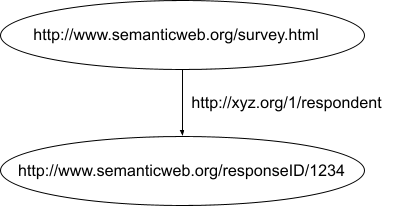
\includegraphics[width=14cm]{images/ch2/Figure10.png}
    \caption{\ac{rdf} Graph for English Statement in Figure~\ref{fig:2.8}, after \ac{rdf} Primer~\cite{manola2004rdf}}
    \label{fig:2.10}
\end{figure}
\par The new graph would be as shown in Figure~\ref{fig:2.11} where as the set of statements in Table~\ref{table:2.2} shows the \ac{rdf} triple notation for Figure~\ref{fig:2.11}. The first notation represents the entities, survey.html (subject) and Robert James (object), along with respondent (predicate) as the relation between them, using the \ac{uri}s. The second notation is for the date, where instead of the \ac{uri}, the value of the property, Sept. 08, 2020, is used. Here, survey.html is the subject and Sept. 08, 2020 is the object with date acting as the predicate.
\begin{figure}[htp]
    \centering
    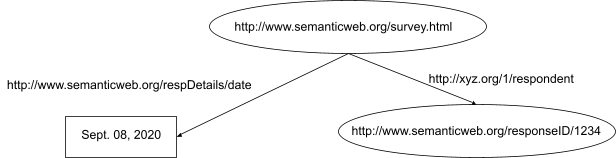
\includegraphics[width=15cm]{images/ch2/Figure11.png}
    \caption{\ac{rdf} Graph for Two Relative Statements, after \ac{rdf} Primer~\cite{manola2004rdf}}
    \label{fig:2.11}
\end{figure}
\begin{table}[h!]
\centering
\begin{tabular}{|l|} 
 \hline
  \ \ <http://www.semanticweb.org/survey.html> <http://xyz.org/1/respondent> \\ \ \ <http://www.semanticweb.org/responseID/1234> . \\ \hline
 \ \ <http://www.semanticweb.org/respDetails/date> “Sept. 08, 2020” . \\ \hline
\end{tabular}
\caption{\ac{rdf} Notations for Figure~\ref{fig:2.11}, after \ac{rdf} Primer~\cite{manola2004rdf}}
\label{table:2.2}
\end{table}
\par Consider a more complex system, where the details of respondent are collected. Suppose, one of the details is name and the other is address of the respondent.  Figure~\ref{fig:2.12} shows a graphical representation of this \ac{rdf} system.
\begin{figure}[htp]
    \centering
    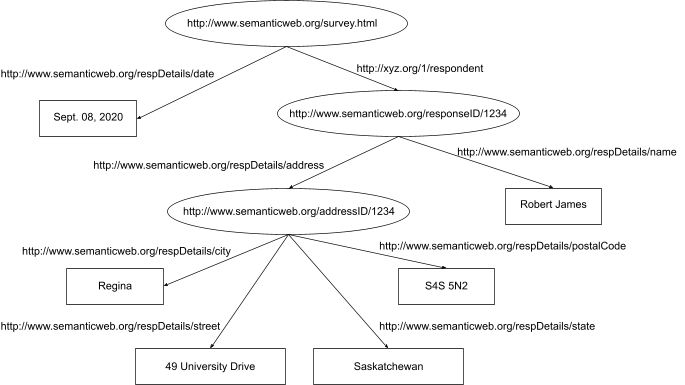
\includegraphics[width=15cm]{images/ch2/Figure12.png}
    \caption{Graphical Representation of \ac{rdf} with Details of the Respondent of the Survey, after \ac{rdf} Primer~\cite{manola2004rdf}}
    \label{fig:2.12}
\end{figure}
%% \marginpar{"after \ac{rdf} Primer" -- this appears a lot. I would like to see  consistency of text sizes and styles, perhaps using \LaTeX directly instead of images...} it is just that the information can be represented in 5 figures and 1 table after reading RDF Primer
\par For name, the respondent is subject and Robert James acts as object whereas respName is the predicate. The \ac{uri} for respName is \say{http://www.semanticweb.org/respDe- tails/name} and the value, Robert James, is the object. On the other hand, respondent (subject) is connected to address (object) node, with \ac{uri} \say{http://www.semanticwe- b.org/addressID/1234}, through respAddress (predicate) with \ac{uri} \say{http://www.sema- nticweb.org/respDetails/address}. Further, the address node has multiple child nodes, namely, street, city, state and postal code. The address (subject) \ac{uri} is connected to the values of four different object values, 49 University Drive (street), Regina (city), Saskatchewan (state) and S4S 5N2 (postalCode) where the \ac{uri}s for the predicates are \say{http://www.semanticweb.org/respDetails/street}, \say{http://www.semanticweb.org/res- pDetails/city}, \say{http://www.semanticweb.org/respDetails/state} and \say{http://www.se- manticweb.org/respDetails/postalCode} respectively. Instead of using an unnecessary \ac{uri} for the address entity, a blank node can be used to denote the entity, as shown in Figure~\ref{fig:2.13}. As the relationships of the node with other nodes give sufficient details without hindering the flow of the data tree, the node does not require a \ac{uri}reference\footnote{https://lists.w3.org/Archives/Public/uri/2007Jul/0027.html}.
\begin{figure}[htp]
    \centering
    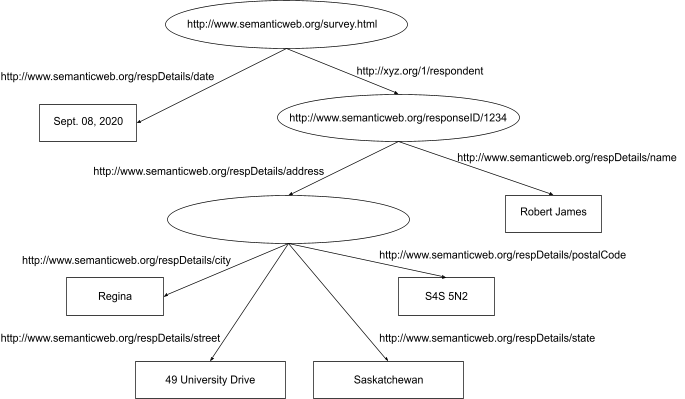
\includegraphics[width=15cm]{images/ch2/Figure13.png}
    \caption{\ac{rdf} Representation in Figure~\ref{fig:2.12} without a URI (blank node) for Address Entity, after \ac{rdf} Primer~\cite{manola2004rdf}}
    \label{fig:2.13}
\end{figure}
\par In 2004, \ac{w3c} recommended intended goals that are to be achieved whenever an \ac{rdf} is to be designed. According to the \ac{w3c}Recommendation\footnote{https://www.w3.org/TR/rdf-concepts/}, the design should \say{have a simple data model; formal semantics and provable inference; should use an extensible \ac{uri}-based vocabulary and an \ac{xml}-based syntax; should support the use of \ac{xml} schema datatypes; and should allow any one to make statements about any resource}.
\subsection{Uniform Resource Identifier} \label{subsection:uri}
\par An abstract (a logical) or a physical resource on the web is identified by a unique set of ASCII characters which is referred to as a \ac{uri}\footnote{https://www.w3.org/wiki/URI}. According to Berners-Lee et. al.~\cite{berners1998uri} in RFC 3986, the unique string, on the web, follows a set of guidelines and security considerations while defining a syntax for the generic \ac{uri} and determining a process for \ac{uri} references' resolution. As mentioned by \ac{w3c}, for the operating systems on \ac{uri}s, some specific \say{protocols are defined depending on the UriScheme\footnote{https://www.w3.org/2001/tag/doc/SchemeProtocols.html}}. A system can perform multiple operations like \say{access}, \say{update}, \say{replace} and \say{find attributes} on the identified resources. In RFC 2396, Berners-Lee et al.~\cite{fielding1998uri} characterized \ac{uri} using three definitions, as shown in Table~\ref{table:2.3}.
\begin{table}[h!]
\centering
\begin{tabular}{| l | l |} 
 \hline
 Term & \ \ \ \ \ \ \ \ \ \ \ \ \ \ \ \ \ \ \ \ \ \ \ \ \ \ \ \ \ \ \ \ \ \ \ \ \ \ \ \ Definition  \\ 
 \hline
  \multirow{9}{4em}{Uniform} & There are various benefits of achieving uniformity, like, it facilitates\\ & different procedures to access resources in the same environment using\\ & different types of resource identifiers; new types of resource identifiers\\ & can be introduced without modifying the actual usage of the existing\\ & identifiers; common syntactic conventions can be interpreted uniformly\\ & for a variety of resource identifiers on the semantic web; and the new\\ & applications or protocols can utilize the already existing large and\\ & widely-used resource identifiers as the identifiers can be reused in\\ & different contexts. \\ \hline
 \multirow{9}{0em}{Resource} & Anything on the web that can be uniquely identified is referred to as\\ & a resource. Some day-to-day examples of a resource are a computeri-\\ & zed file or folder, weather-broadcasting service, an image, and a set of\\ & other resources. Some resources like books in a library, an animal, a\\ & human being,and a corporation are a set of resources that cannot be\\ & retrieved over the network. A resource is the \say{conceptual mapping}\\ &~\cite{fielding1998uri} to a set of entities independent of the corresponding entities at a\\ & particular time. Hence, if the conceptual mapping isn't changed, a\\ & resource can remain constant irrespective of the changes in its content.\\ \hline
 \multirow{3}{0em}{Identifier} & An object which is used as a reference to a thing with unique identity\\ & on the web is termed as an identifier. In \ac{uri}, a string of ASCII char-\\ & acters restricted by a specific syntax is object.\\ \hline
\end{tabular}
\caption{Definitions Used for Characterizing URI, by Berners-Lee et al.~\cite{fielding1998uri}}
\label{table:2.3}
\end{table}  
\subsubsection{Syntax of a \ac{uri}}
\par According to Berners-Lee et al.~\cite{berners1998uri}, the generic syntax of a \ac{uri} comprises five components in a hierarchical sequence which are as follows:
\begin{center}
\par \ac{uri} = scheme: [//authority] path [?query] [\#fragment]    
\end{center}
where the authority component consists of three more components which are:
\begin{center}
\par authority = [userinfo@] host [:port]
\end{center}
\par A syntax diagram can be modelled to represent the components of Generic Syntax\footnote{https://www.w3.org/Addressing/URL/uri-spec.html} of \ac{uri} along with their hierarchy as shown in Figure~\ref{fig:2.14}. Consider the following \ac{url}. Figure~\ref{fig:2.15} shows its components.
\begin{center}
\par https://parita@www.semanticweb.org:695/ontology/?tag=survey\&order=newest\#top
\end{center}
\begin{figure}[htp]
    \centering
    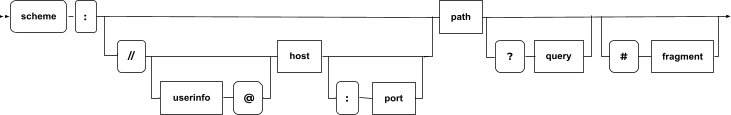
\includegraphics[width=15cm]{images/ch2/Figure14.png}
    \caption{Syntax Diagram of a Generic URI, after Berners-Lee et al.~\cite{berners1998uri}}
    \label{fig:2.14}
\end{figure}
\begin{figure}[htp]
    \centering
    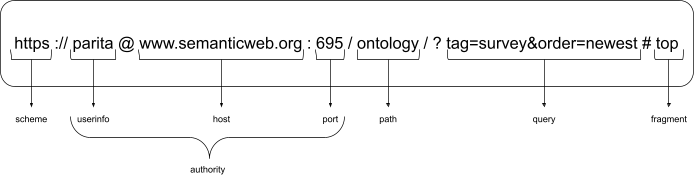
\includegraphics[width=15cm]{images/ch2/Figure15.png}
    \caption{Components of an Example of URL, after Berners-Lee et al.~\cite{berners1998uri}}
    \label{fig:2.15}
\end{figure}
\section{Linked Data Life Cycle}
\par The Linked Data Life Cycle includes multiple stages as described by Ngomo et al.~\cite{ngomo2014introduction} which are listed in Table~\ref{table:2.4}. Each stage of this life cycle is independent yet linked to one another. So, it is not mandatory to go through all the stages sequentially to publish the data on the web. It is necessary to use a procedure that follows the life cycle to ensure the quality of data to be published as linked data. The first stage, generally, is data extraction along with conversion of the extracted data (in forms other than \ac{rdf}) into \ac{rdf}. Once the data is in \ac{rdf} form, any or all of the other stages listed in Table~\ref{table:2.4} can be performed.
\begin{table}[h!]
    \centering
    \begin{tabular}{|l|l|} 
    \hline Stage \ & Description \\ \hline
     Extraction & Extraction and conversion of unstructured and semi-\\ & structured data into \ac{rdf}\\ \hline
     Storage \& Querying & Storing the \ac{rdf} data in a format that supports data\\ & querying efficiently\\ \hline
     Authoring & Allowing the users to create new data or to access and\\ & modify the existing data\\ \hline
     Linking & Creating links the data belonging to various domains\\ & and users based on their entities\\ \hline
     Enrichment & Data enrichment for efficient query support using\\ & various top-tier structures\\ \hline
     Quality Analysis & Managing data using different strategies to ensure good\\ & quality of available data on the web\\ \hline
     Browsing \& Exploration & Making the structured data available on the web for\\ & the users to browse and explore effectively\\ \hline
    \end{tabular}
    \caption{Stages in Linked Data Life Cycle, after Ngomo et al.~\cite{ngomo2014introduction}}
    \label{table:2.4}
    \end{table}
\section{Conversion of Data from CSV to \ac{rdf}}
\par The preferred format of the data published on the semantic web is \ac{rdf} format. Many data scientists use tables and spreadsheets to store and publish data using \ac{csv} files over \ac{rdf} format as conversion of data to \ac{rdf} is comparatively difficult. The data used by Dr. Hepting has been stored in tabular format (Sample \ac{csv} data consisting of all responses is available in Appendix~\ref{chap:appendix1} ). To convert tabular data into \ac{rdf} (Appendix~\ref{chap:appendix2} consists of \ac{rdf} code for the \ac{csv} data in Appendix~\ref{chap:appendix1}), \ac{w3c}\footnote{https://www.w3.org/wiki/ConverterToRdf} recommends the following open source tools~\cite{ermilov2013csv},
\begin{itemize}
    \item OpenRefine:
    \par OpenRefine\footnote{https://openrefine.org}, an \ac{rdf} extension of Google Refine, is a powerful java-based set of tools that work with messy data using \ac{grel}\footnote{https://libjohn.github.io/openrefine/grel.html}. It allows the users to extract, transform, export, and convert \ac{csv}, Ex cel, spreadsheets and other tabular data into \ac{rdf} where a \ac{gui} is used to define schema mapping.
    \item RDF123:
    \par RDF123\footnote{https://ebiquity.umbc.edu/resource/html/id/237/RDF123-java-application-v1-0} is a java application and servlet for the conversion of \ac{csv} and spreadsheets to \ac{rdf} which uses arbitrary graphs to define schema mapping. According to Han et. al~\cite{han2008rdf}, it uses a graphical RDF123 template to allow users to convert the data from spreadsheets to \ac{rdf}.
    \item csv2rdf4lod:
    \par csv2rdf4lod\footnote{https://github.com/timrdf/csv2rdf4lod-automation/wiki} is a tool that is used for the conversion of tabular data into structured and linked \ac{rdf} using specifications that are based on declarative \ac{rdf} enhancement parameters. It forms default namespaces for \ac{uri}s and provides VoID and original metada for the conversion using identifiers for source organization, dataset and version.
    \item XLWrap:
    \par XLWrap\footnote{https://xlwrap.sourceforge.io} is a graphical template based application that allows execution of various \ac{sparql} queries~\cite{andreas2009xlwrap}.  The spreadsheets are wrapped to arbitrary \ac{rdf} graphs which allows:
    \begin{itemize}
    	\item Streamed processing of tabluar data like Excel, OpenDocument and \ac{csv}
	\item Loading Local/\ac{http}
	\item Expressions that include calculator operations for Excel and OpenDocument, and Custom functions
	\item Use of \ac{api} and \ac{sparql} endpoint
    \end{itemize}
    \item Tarql:
    \par Tarql\footnote{https://tarql.github.io} operates as a command-line application for the conversion of \ac{csv} to \ac{rdf} using a user-defined mapping that is written in \ac{sparql} standard 1.1.
\end{itemize}
\section{Ontology Editors}
\par Ontology editors are used by publishers to create new ontologies when the existing vocabulary is not suitable for their purpose. \ac{w3c}\footnote{https://www.w3.org/wiki/Ontology\_editors} has recommended a list of ontology editors that can be used to edit, manage, organize and visualize ontology. The list of editors includes Protégé, NeOn Toolkit, SWOOP, Neologism, TopBraid Composer, Vitro, Knoodl, Anzo for Excel, OWLGrEd, Fluent Editor, Semantic Turkey, VocBench. The page does not include valid links to the editors' websites. Protégé is the most popular ontology editor among researchers. There exists negligible information about most of the editors in the list which has driven the decision of the use of Protégé for ontology development and OntoGraf and WebVOWL for visualization.
\section{Applications of Linked Open Data}
\par A variety of projects and websites, that use linked open data, have been developed. Wikidata and DBpedia are two major projects of linked open data that present structured data on the semantic web. This section consists of a brief description of both applications.
\subsection{Wikidata}
\par According to a report by Krotzsch and Vrandecic~\cite{denny2014wikidata}, Wikidata was introduced to the world of information engineering in 2012 by Wikimedia. Wikidata can be defined as \say{the community-created
knowledge base of Wikipedia and the central data management platform for
Wikipedia and most of its Sister Projects\footnote{Wikipedia, Wikivoyage, Wiktionary, Wikisource, and others}}, according to Erxleben et al.~\cite{fredo2014intro}. Wikidata was established for the collection and integration of data on the semantic web with Wikipedia. Wikidata is a free open-source tool that handles a large amount of structured data and maintains pages that store the data. Each entity on Wikidata represents the subject of a triple with a dedicated page. The properties of Wikidata are similar to that of \ac{rdf} where the individuals and classes are indicated using items. As Wikidata is an open-source tool, the data on a page of the Wikidata is easily available for the users to access as well as edit.
\par For instance, the University of Regina, a university in the provincial capital of Saskatchewan—the city of Regina, has an item page allotted for it. Figure~\ref{fig:2.16} shows the Wikidata item page of the University of Regina that can be accessed using the link: https://www.wikidata.org/wiki/Q3104287. Wikidata uses a method of automatically assigning unique identifiers to the entities, which are used as the labels of the item pages instead of the actual names of the entities. These identifiers are a string starting with a capital Q followed by a sequence of digits. The identifiers are assigned irrespective of the language as the Wikidata website supports multiple languages. For the University of Regina, the label used is \say{Q3104287}. The item page on Wikidata consists of multiple sections:
\begin{itemize}
    \item label: The name of the subject that is treated as an entity. For the instance in Figure~\ref{fig:2.16}, the label is \say{University of Regina} along with the unique identifier \say{Q3104287}. 
    \begin{figure}[htp]
    \centering
    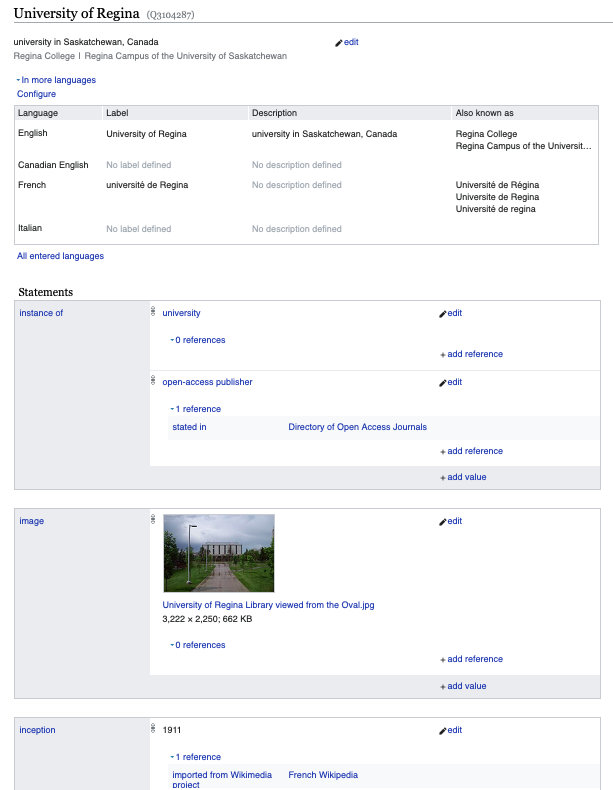
\includegraphics[width=15cm]{images/ch2/Figure16.png}
    \caption{Details of University of Regina, Regina, SK on Wikidata}
    \label{fig:2.16}
\end{figure}
    \item description: This section consists of general introductory details about the subject. For the University of Regina, the description on wikidata is \say{university in Saskatchewan, Canada}.
    \item statements: This section consists of a list of subsections called \say{property}. The properties along with their property IDs for the University of Regina are listed in Table~\ref{table:2.5}.
    \begin{table}[h!]
    \centering
    \begin{tabular}{|l|l|} 
    \hline Statement Property \ & Property ID \\ \hline
     instance of & P31\\ \hline
     image & P18\\ \hline
     inception & P571\\ \hline
     country & P17\\ \hline
     located in the administrative territorial entity & P131\\ \hline
     coordinate location & P625\\ \hline
     subsidiary & P355\\ \hline
     official website & P856\\ \hline
     commons category & P373\\ \hline
     topic's main category & P910\\ \hline
     category for employees of the organization & P4195\\ \hline
     category for alumni of educational institution & P3876\\ \hline
     API endpoint & P6269\\ \hline
     social media followers & P8687\\ \hline
    \end{tabular}
    \caption{Statement Properties and Property IDs for the University of Regina on Wikidata}
    \label{table:2.5}
    \end{table}
    \item identifiers: This section consists of various IDs belonging to the subject. For the University of Regina, the set of properties used for identifiers and their IDs are listed in Table~\ref{table:2.6}.
    \begin{table}[h!]
    \centering
    \begin{tabular}{|l|l|} 
    \hline Identifier Property \ & Property ID \\ \hline
     VIAF ID & P214\\ \hline
     ISNI & P213\\ \hline
     GND ID & P227\\ \hline
     Library of Congress authority ID & P244\\ \hline
     WorldCat Identities & P7859\\ \hline
     ARWU university ID & P5242\\ \hline
     Crossref funder ID & P3153\\ \hline
     Facebook ID & P2013\\ \hline
     Freebase ID & P646\\ \hline
     Google Maps Customer ID & P3749\\ \hline
     GRID ID & P2427\\ \hline
     HAL structure ID & P6773\\ \hline
     LittleSis organization ID & P3393\\ \hline
     Microsoft Academic ID & P6366\\ \hline
     Ringgold ID & P3500\\ \hline
     ROR ID & P6782\\ \hline
     Times Higher Education World University ID & P5586\\ \hline
     Twitter username & P2002\\ \hline
     U-Multirank university ID & P5600\\ \hline
    \end{tabular}
    \caption{Identifier Properties and Property IDs for University of Regina on Wikidata}
    \label{table:2.6}
    \end{table}
\end{itemize}
\par The \ac{uri} for an entity on Wikidata is \say{https://www.wikidata.org/wiki/<id>}, where <id> stands for the unique identifier. For the University of Regina, the <id> is the label identifier—Q3104287. Figure~\ref{fig:2.17} shows the \ac{rdf}/\ac{xml} description of the University of Regina on Wikidata.
\begin{figure}[htp]
    \centering
    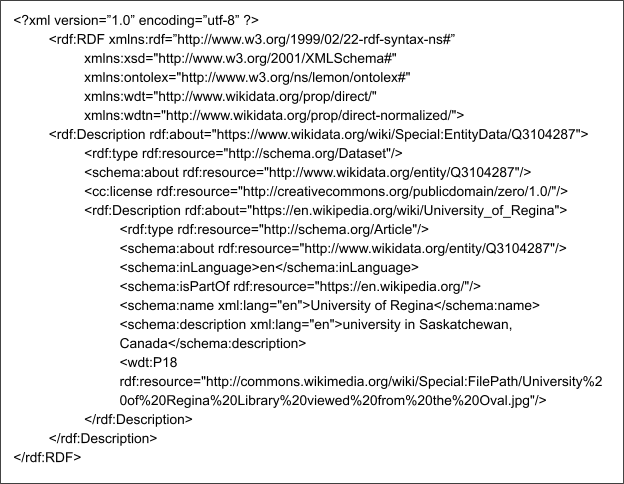
\includegraphics[width=15cm]{images/ch2/Figure17.png}
    \caption{Wikidata Entry (RDF/XML) for University of Regina, Regina, SK}
    \label{fig:2.17}
\end{figure}
\subsection{DBpedia}
\par Jimmy Wales and Larry Sanger, in 2001, created the largest general reference work on the internet consisting of articles\footnote{include data comprising of templates, images, videos, categorizations, and links to other articles (pages) in multiple languages} in over 280 languages, the Wikipedia\footnote{https://en.wikipedia.org/wiki/Main\_Page}, which acts as a source of data for many web projects like DBpedia\footnote{https://wiki.dbpedia.org/}, one of the major linked open data projects. The main aim behind the development of DBpedia is the conversion of unstructured data on Wikipedia into structured datasets. DBpedia enables querying the Wikipedia data as well as the generation of links among the structured datasets, resulting in the establishment of a massive web of data.
\par Initially, the template of the page is discovered using a Template Extraction Algorithm\footnote{like Principle Components Analysis, Linear Discriminant Analysis, Logically Linear Embedding} which results in the identification of the structure of the template using various Pattern Matching Techniques\footnote{https://www.dummies.com/programming/big-data/data-science/how-pattern-matching-works-in-data-science}. Once the appropriate template is selected, the template data is parsed using a suitable algorithm and transformed into \ac{rdf} triples. MediaWiki\footnote{https://www.mediawiki.org/wiki/MediaWiki} links are identified and assigned specific \ac{uri}s. On the other hand, the common units of data are recognized  and assigned appropriate datatypes whereas \ac{rdf} lists are created for the object lists. According to Auer et al.~\cite{auer2007dbpedia}, DBpedia in 2007 was a platform that delivered information on \say{more than 1.95 million \say{things} that includes at least 80,000 persons, 70,000 places, 35,000 music albums, 12,000 films}. The DBpedia semantic web services are handled using the GNU Free Documentation License terms and policies. The data on DBpedia is easily accessible in different ways like accessing the datasets as linked data; using \ac{sparql} queries for data extraction and accessibility; and in the form of a downloadable \ac{rdf} snippets~\cite{bizer2009dbpedia}. Figure~\ref{fig:2.18} shows DBpedia entry for the \say{University of Regina, Regina, SK}. Like Wikidata, DBpedia also has a label, a description section and a set of important property-value pairs that give information related to the entity that has been described.
\begin{figure}[htp]
\centering
    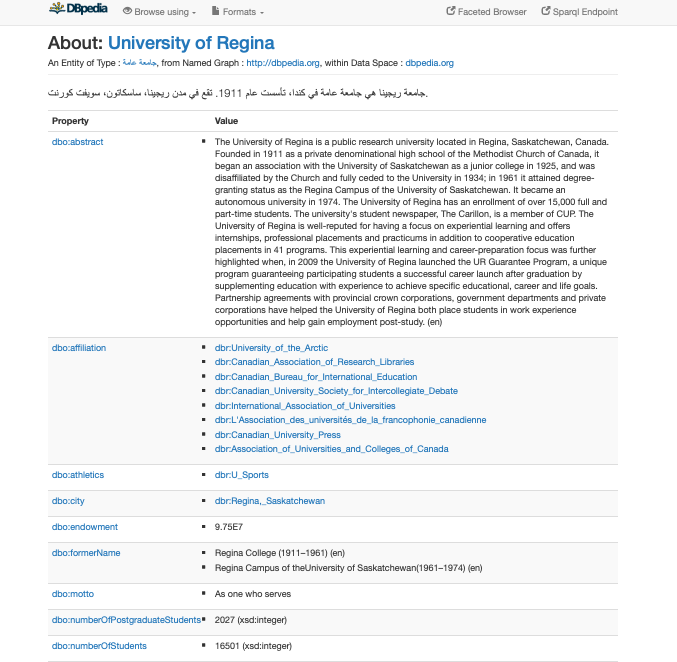
\includegraphics[width=15cm]{images/ch2/Figure18.png}
    \caption{Description of University of Regina, Regina, SK on DBpedia}
    \label{fig:2.18}
\end{figure}
\par Figure~\ref{fig:2.19} shows the data architecture of DBpedia. An open-link software, Virtuoso Universal Server\footnote{https://dbpedia.org/page/Virtuoso\_Universal\_Server}, is a data virtualization tool used to host and publish \ac{rdf} datasets on DBpedia, which can be easily accessed using \ac{sparql} endpoint. The \ac{html} or \ac{rdf} representation of the DBpedia resources is enabled by the data architecture using \ac{http} that supports the standard \ac{http} GET method calls from the web clients.
\begin{figure}[htp]
    \centering
    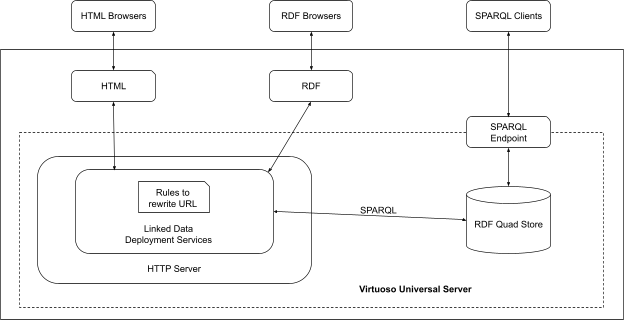
\includegraphics[width=15cm]{images/ch2/Figure19.png}
    \caption{DBpedia Data Architecture}
    \label{fig:2.19}
\end{figure}
\end{doublespace}


